\subsection{API}
Selanjutnya kita akan membuat APInya menggunakan PHP. Persiapkan terlebih dahulu folder dan file yang nantinya kita butuhkan dalam pembuatan APInya. Pertama kita buat folder dosen, images, mahasiswa, dan pembimbing. Lalu kita buat juga file config.php dan conn.php.

\begin{figure}[H]
\centering
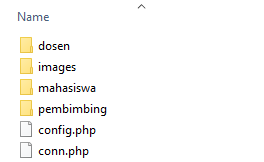
\includegraphics[width=4.2cm]{figures/api/api1.png}
\end{figure}

\noindent
Lalu di dalam folder dosen buat beberapa file sebagai berikut.

\begin{figure}[H]
\centering
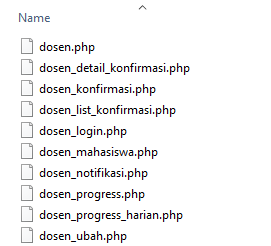
\includegraphics[width=4.2cm]{figures/api/api2.png}
\end{figure}

\noindent
Kemudian di dalam folder mahasiswa buat beberapa file sebagai berikut.

\begin{figure}[H]
\centering
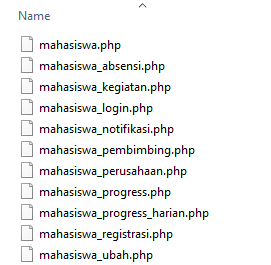
\includegraphics[width=4.2cm]{figures/api/api3.png}
\end{figure}

\noindent
Selanjutnya di dalam folder pembimbing buat beberapa file sebagai berikut.

\begin{figure}[H]
\centering
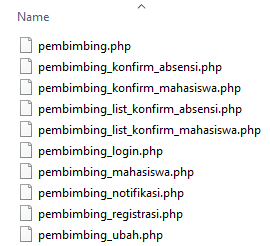
\includegraphics[width=4.2cm]{figures/api/api4.png}
\end{figure}

\noindent
Setelah itu, di dalam folder images buat beberapa folder sebagai berikut.

\begin{figure}[H]
\centering
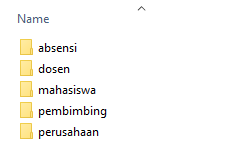
\includegraphics[width=4.2cm]{figures/api/api5.png}
\end{figure}

\noindent
Kemudian tambahkan script berikut di file config.php
\lstinputlisting[language=PHP]{src/actspotapi/config.php}

\noindent
Selanjutnya tambahkan script berikut di file conn.php
\lstinputlisting[language=PHP]{src/actspotapi/conn.php}

\noindent
Setelah itu, tambahkan script berikut di file dosen.php pada folder dosen.
\lstinputlisting[language=PHP]{src/actspotapi/dosen/dosen.php}

\noindent
Kemudian tambahkan script berikut di file dosen\_detail\_konfirmasi.php pada folder dosen.
\lstinputlisting[language=PHP]{src/actspotapi/dosen/dosen_detail_konfirmasi.php}

\noindent
Selanjutnya tambahkan script berikut di file dosen\_konfirmasi.php pada folder dosen.
\lstinputlisting[language=PHP]{src/actspotapi/dosen/dosen_konfirmasi.php}

\noindent
Setelah itu, tambahkan script berikut di file dosen\_list\_konfirmasi.php pada folder dosen.
\lstinputlisting[language=PHP]{src/actspotapi/dosen/dosen_list_konfirmasi.php}

\noindent
Kemudian tambahkan script berikut di file dosen\_login.php pada folder dosen.
\lstinputlisting[language=PHP]{src/actspotapi/dosen/dosen_login.php}

\noindent
Selanjutnya tambahkan script berikut di file dosen\_mahasiswa.php pada folder dosen.
\lstinputlisting[language=PHP]{src/actspotapi/dosen/dosen_mahasiswa.php}

\noindent
Setelah itu, tambahkan script berikut di file dosen\_notifikasi.php pada folder dosen.
\lstinputlisting[language=PHP]{src/actspotapi/dosen/dosen_notifikasi.php}

\noindent
Kemudian tambahkan script berikut di file dosen\_progress\_harian.php pada folder dosen.
\lstinputlisting[language=PHP]{src/actspotapi/dosen/dosen_progress_harian.php}

\noindent
Selanjutnya tambahkan script berikut di file dosen\_progress.php pada folder dosen.
\lstinputlisting[language=PHP]{src/actspotapi/dosen/dosen_progress.php}

\noindent
Setelah itu, tambahkan script berikut di file dosen\_ubah.php pada folder dosen.
\lstinputlisting[language=PHP]{src/actspotapi/dosen/dosen_ubah.php}

\noindent
Kemudian tambahkan script berikut di file mahasiswa.php pada folder mahasiswa.
\lstinputlisting[language=PHP]{src/actspotapi/mahasiswa/mahasiswa.php}

\noindent
Selanjutnya tambahkan script berikut di file mahasiswa\_absensi.php pada folder mahasiswa.
\lstinputlisting[language=PHP]{src/actspotapi/mahasiswa/mahasiswa_absensi.php}

\noindent
Setelah itu, tambahkan script berikut di file mahasiswa\_kegiatan.php pada folder mahasiswa.
\lstinputlisting[language=PHP]{src/actspotapi/mahasiswa/mahasiswa_kegiatan.php}

\noindent
Kemudian tambahkan script berikut di file mahasiswa\_login.php pada folder mahasiswa.
\lstinputlisting[language=PHP]{src/actspotapi/mahasiswa/mahasiswa_login.php}

\noindent
Selanjutnya tambahkan script berikut di file mahasiswa\_notifikasi.php pada folder mahasiswa.
\lstinputlisting[language=PHP]{src/actspotapi/mahasiswa/mahasiswa_notifikasi.php}

\noindent
Setelah itu, tambahkan script berikut di file mahasiswa\_pembimbing.php pada folder mahasiswa.
\lstinputlisting[language=PHP]{src/actspotapi/mahasiswa/mahasiswa_pembimbing.php}

\noindent
Kemudian tambahkan script berikut di file mahasiswa\_perusahaan.php pada folder mahasiswa.
\lstinputlisting[language=PHP]{src/actspotapi/mahasiswa/mahasiswa_perusahaan.php}

\noindent
Selanjutnya tambahkan script berikut di file mahasiswa\_progress\_harian.php pada folder mahasiswa.
\lstinputlisting[language=PHP]{src/actspotapi/mahasiswa/mahasiswa_progress_harian.php}

\noindent
Setelah itu, tambahkan script berikut di file mahasiswa\_progress.php pada folder mahasiswa.
\lstinputlisting[language=PHP]{src/actspotapi/mahasiswa/mahasiswa_progress.php}

\noindent
Kemudian tambahkan script berikut di file mahasiswa\_registrasi.php pada folder mahasiswa.
\lstinputlisting[language=PHP]{src/actspotapi/mahasiswa/mahasiswa_registrasi.php}

\noindent
Selanjutnya tambahkan script berikut di file mahasiswa\_ubah.php pada folder mahasiswa.
\lstinputlisting[language=PHP]{src/actspotapi/mahasiswa/mahasiswa_ubah.php}

\noindent
Setelah itu, tambahkan script berikut di file pembimbing.php pada folder pembimbing.
\lstinputlisting[language=PHP]{src/actspotapi/pembimbing/pembimbing.php}

\noindent
Kemudian tambahkan script berikut di file pembimbing\_konfirm\_absensi.php pada folder pembimbing.
\lstinputlisting[language=PHP]{src/actspotapi/pembimbing/pembimbing_konfirm_absensi.php}

\noindent
Selanjutnya tambahkan script berikut di file pembimbing\_konfirm\_mahasiswa.php pada folder pembimbing.
\lstinputlisting[language=PHP]{src/actspotapi/pembimbing/pembimbing_konfirm_mahasiswa.php}

\noindent
Setelah itu, tambahkan script berikut di file pembimbing\_list\_konfirm\_absensi.php pada folder pembimbing.
\lstinputlisting[language=PHP]{src/actspotapi/pembimbing/pembimbing_list_konfirm_absensi.php}

\noindent
Kemudian tambahkan script berikut di file pembimbing\_list\_konfirmasi\_mahasiswa.php pada folder pembimbing.
\lstinputlisting[language=PHP]{src/actspotapi/pembimbing/pembimbing_list_konfirm_mahasiswa.php}

\noindent
Selanjutnya tambahkan script berikut di file pembimbing\_login.php pada folder pembimbing.
\lstinputlisting[language=PHP]{src/actspotapi/pembimbing/pembimbing_login.php}

\noindent
Setelah itu, tambahkan script berikut di file pembimbing\_mahasiswa.php pada folder pembimbing.
\lstinputlisting[language=PHP]{src/actspotapi/pembimbing/pembimbing_mahasiswa.php}

\noindent
Kemudian tambahkan script berikut di file pembimbing\_notifikasi.php pada folder pembimbing.
\lstinputlisting[language=PHP]{src/actspotapi/pembimbing/pembimbing_notifikasi.php}

\noindent
Selanjutnya tambahkan script berikut di file pembimbing\_registrasi.php pada folder pembimbing.
\lstinputlisting[language=PHP]{src/actspotapi/pembimbing/pembimbing_registrasi.php}

\noindent
Setelah itu, tambahkan script berikut di file pembimbing\_ubah.php pada folder pembimbing.
\lstinputlisting[language=PHP]{src/actspotapi/pembimbing/pembimbing_ubah.php}
